\chapter{Modellierung}
\label{sec:modellierung}
Im mathematischen Modell werden die Anforderungen aus der Trainingswissenschaft in das Format der Constraint Programmierung übersetzt. Die Modellierung löst jeden Monat gesondert und berechnet deshalb die Trainingseinheiten für einen Zeitraum von 28 Tagen. Dauer, Methode und Belastungsbereiche charakterisieren eine Einheit. Später werden die Mesozyklen dann zu einem Makrozyklus verbunden, der den gesamten Trainingsplan widerspiegelt.

\section{Prozess}
Im ersten Ansatz der Modellierung eines Trainingsplans wurden kein kombinatorischer Grundgedanke verfolgt. Statt eines Pools an validen Trainingseinheiten, definierte das System die Charakteristika einer Trainingsmethode. Die Schwierigkeit ist jedoch die vielen Einzelfälle und Ausnahmen präzise genug abzudecken ohne ein sehr unübersichtliches Constraint-System zu erhalten. Besonders im Hinblick auf die Erweiterung und Skalierbarkeit scheiterte dieser Versuch. Stattdessen wird das Problem als kombinatorische Optimierung betrachtet, das die einzelnen Trainingsmethoden mit dynamischer Verteilung der Belastungsbereiche definiert. Ein weiterer Vorteil ist die einfache Erweiterung um weitere Arten von Trainingseinheiten. Die Benennung in der Liste der annehmbaren Verteilungen konkretisiert sich auch die Darstellung in der Ausgabe. \par
Des Weiteren wurde von einer Modellierung auf Basis von Kraft, Ausdauer und Schnelligkeitsanteilen abgesehen. In diesem Fall wären Schätzungen an zwei Stellen vonnöten. Erst müssen für die Trainingseinheiten die drei Bereiche festgelegt werden und dann, wie auch in der aktuellen Modellierung, die Gewichtung in Abhängigkeit der Wettkampfsdisziplin. Mit Definition einer Trainingseinheit über die Belastungsbereiche selbst, kann die Abschätzung an einer Stelle gebündelt werden. Die Wettkampfsarten dienen als Vorlage für die Verteilung, sind von der Modellierung aber unabhängig festgelegt.\par
Die Optimierung auf Ebene der Mesozyklen erlaubt der Verteilung und Variation genug Spielraum. Die Gefahr einer wochenweisen Optimierung ist, dass es eine Lösungsinstanz gibt, die für alle Wochen in sehr ähnlicher Form verwendet wird. Die Variation lässt sich damit nicht genügend steuern. Anhand der monatlichen Kapselung wirkt man der Monotonie entgegen und die Erstellung eines Trainingsplans kann dennoch in ausreichend kleine Teilprobleme zerlegt werden.

\section{Model}
\label{sec:modellierung:model}
% \section{Verfahrensweise}
% \label{sec:modellierung:uebersicht}
% \begin{figure}[htb]
% 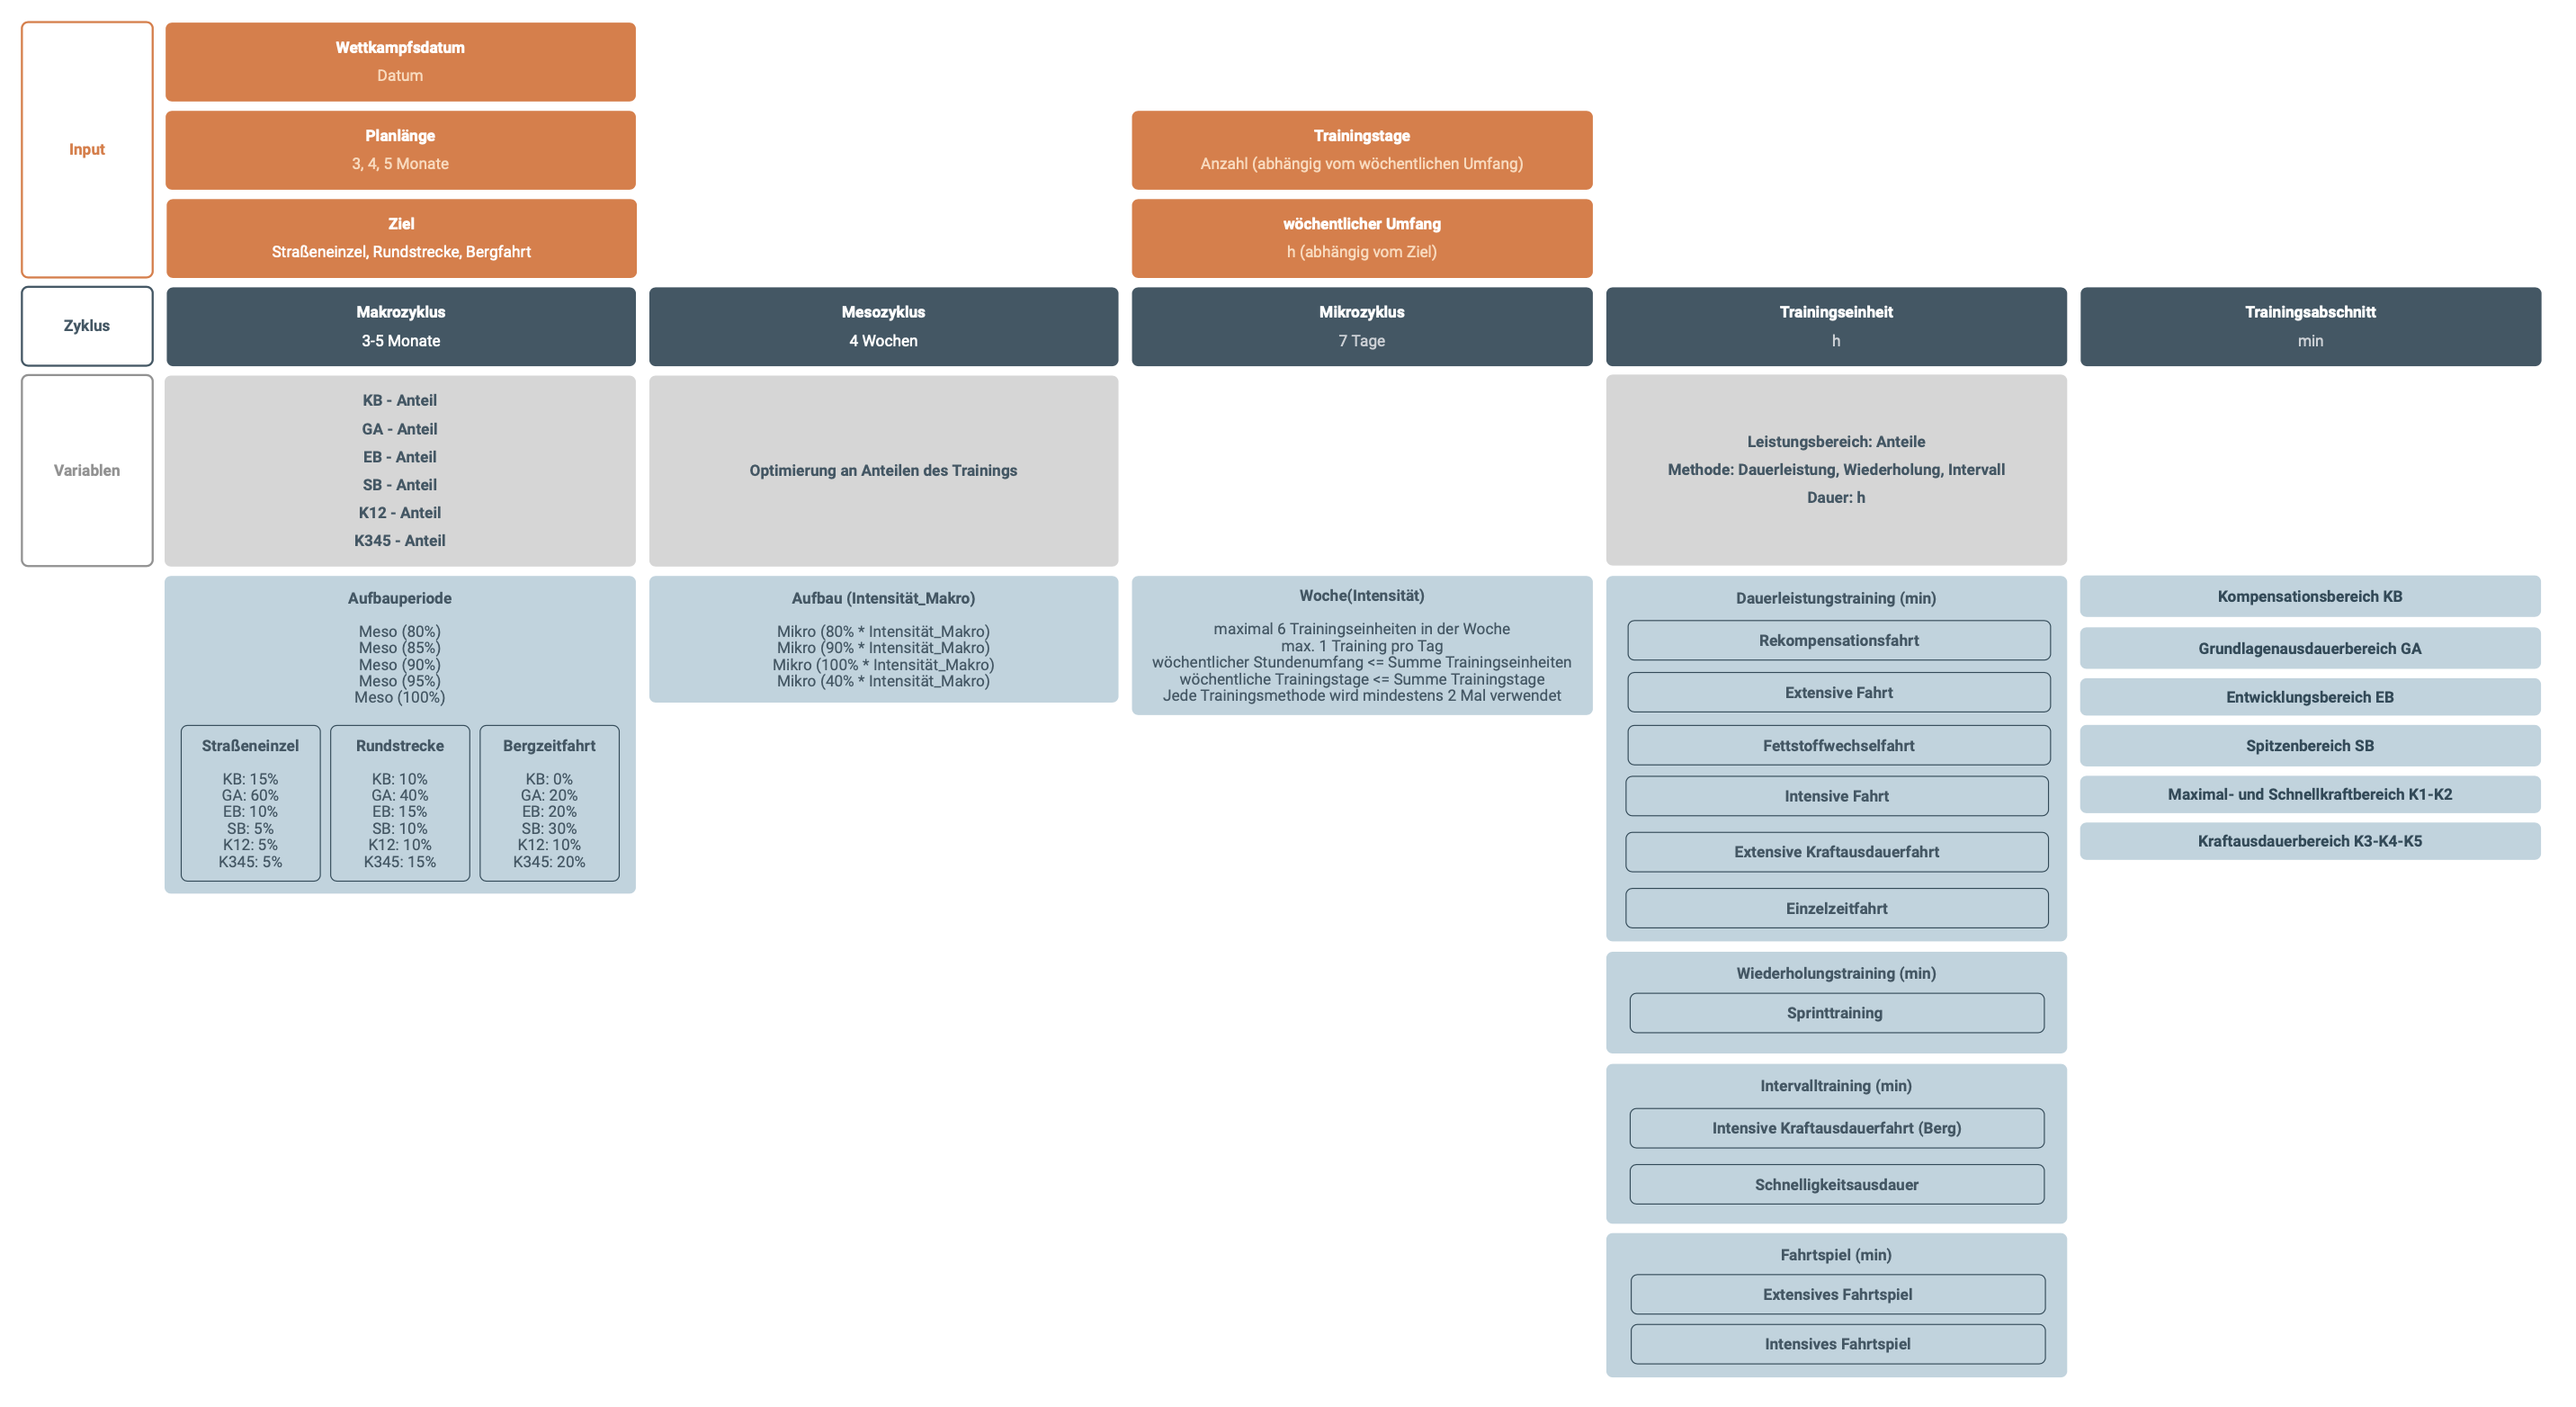
\includegraphics[width=\textwidth]{gfx/modellierung.png}
% \caption{Schema aus Makro-, Meso- und Mikrozyklen}
% \label{fig:modellierung:schema}
% \end{figure}

%\begin{enumerate}
%    \item Die vier Wochen des Mesozyklus progressiv gestalten mit einer 3:1 Periodisierung 
%    \item Trainingsziel und Länge des Plans bestimmen die wöche
%    \item Jeden Monat des Trainingplans einzeln lösen
%    \item Constraints auf Ebene der Hierarchie definieren 
%    \item Solver parallelisiert für jeden Mesozyklus starten
%    \item Trainingseinheiten aus den Mesozyklen zu einem Trainingsplan zusammensetzen
%\end{enumerate}

\subsection{Konstanten}
In der Modellierung betrachten wir Konstanten gesondert. Diese Größen sind in jeder Lösungsinstanz relevant aber vor der Modellierung fest bestimmt.

In $maxminutes_i$ sind die Beschränkung der Trainingsminuten der vier Wochen ($ i \in [ 1, 4]$) festgesetzt. In diesem Modell wird eine Trainingswoche auf maximal 15 Stunden begrenzt. Bereits vor dem Lösen des Modell ist die 3:1 Periodisierung in diesen Variablen festgehalten. Die vier Wochen des Mesozyklus werden nach dem Schema progressiv gestaltet. Die Trainingsminuten betragen 80\%, 90\%, 100\%, 70\% Prozent des Umfangs ihres Makrozyklus. Mit dieser Methode ist auch sichergestellt, dass zum Ende des Plans -- und damit in der Woche vor dem Wettkampf -- eine Regenerationswoche eingeplant wird.
\begin{equation}
     maxminutes_i \in [0, 900] 
\end{equation}


Analog dazu gibt es auch eine Begrenzung der Trainingstage einer Woche. Die Anforderung an mindestens einen Regenerationstag ist hier umgesetzt, da die Trainingstage nicht sieben Tage betragen können. Dieses Limit gilt für jede der 4 Wochen.
\begin{equation}
\label{equation:maxDays}
     maxdays \in [2, 6]
\end{equation}

Maßgeblich für die Optimierungsvariable sind die festgesetzten Ziele je Belastungsbereich. Sie werden aus den Anforderungen eines Wettkampfs und den zur Verfügung stehenden Trainingsminuten berechnet. Wichtig ist hier die zyklischen Wochenumfänge prozentual einzubeziehen, damit die vorgegebenen Minuten in den Bereichen auch mit den wöchentlichen Begrenzungen erreichbar sind.\newline
Auch die Periodisierung des Trainingsplans kann damit gesteuert werden. Je näher die Monate am Wettkampfsdatum liegen, desto höher wird die Wettkampfspezifische Belastung gewichtet. Auch dieses Prinzip wird schon vor der Modellierung durch den Makrozyklus umgesetzt.
\begin{equation}
    kb, ga, eb, sb, k1, k4 \in [0, 900*4]
\end{equation}

\subsection{Variablen}
Unter den Variablen der Modellierung versteht man die veränderlichen Größen. Die endlichen Wertebereiche sind möglichst präzise zu wählen, um den Suchraum verkleinern. Eine Lösungsinstanz definiert die Belegung der Variablen mit konkreten Werten für jeden Tag des Mesozyklus, $\forall i \in [1, 28]$.\par
\textbf{Name der Trainingseinheit} \\[0.2em]
Variable für die Identifikation der Trainingseinheit am Tag $i$. Die Liste der Trainingseinheiten wird durch eine 1:1-Korrespondenz (siehe \ref{anhang:trainingsarten}) abgebildet.
\begin{equation}
    name_i = [\![0, 11]\!]
\end{equation}
\textbf{Dauer einer Einheit} \\[0.2em]
Variable für die Dauer der Trainingseinheit an Tag $i$ in Minuten. Es wird für einen Tag eine maximale Trainingszeit von 6 Stunden angesetzt.
\begin{equation} 
    duration_i = [\![0, 360]\!] \end{equation} 
\textbf{Trainingsmethode einer Einheit} \\[0.2em]
Variable für die Trainingsmethode der Trainingseinheit an Tag $i$. Für Tage ohne Trainingseinheit wird die Methode \textit{PAUSE} eingeführt. Auch wenn aus dem Namen der Trainingseinheit ein direkter Zusammenhang mit der Methode besteht, wird diese explizit definiert, um die Variation der Trainingsmethoden zu gewährleisten.
\begin{equation}
    method_i = \{\text{PAUSE, DL, FS, IV, WH}\}
\end{equation} 
\textbf{Leistungsbereiche einer Einheit} \\[0.2em]
Variable für die Minuten je Belastungsbereich an Tag $i$. Die maximale Trainingszeit gilt hier gleichermaßen, da ein Training bei der Dauerleistungsmethode in nur einem Bereich absolviert wird. \newline
\begin{equation} 
\begin{array}{c}
    kb_i = [\![0, 360]\!] \\
    ga_i = [\![0, 360]\!] \\
    eb_i = [\![0, 360]\!] \\
    sb_i = [\![0, 360]\!] \\
    k1_i = [\![0, 360]\!] \\
    k4_i = [\![0, 360]\!] \\
\end{array}
\end{equation} 
\subsection{Constraints}
\textbf{Diskretisierung der Trainingseinheiten} \\[0.2em]
Die Trainingseinheiten werden bei ihrer Länge auf viertelstündliche Abschnitte diskretisiert. Das verkleinert den Wertebereich der Variable um 93,3\% und die Trainingseinheiten sind im Hinblick auf den Anwendungsfall praxistauglich.
\begin{equation}
    {duration}_i \mod 15 = 0 , \forall i \in [1, 28]
\end{equation} 
\textbf{Diskretisierung der Trainingsbereiche} \\[0.2em]
Vergleichbar sind Trainingsbereiche einer Einheit in fünf Minuten Abschnitten festgesetzt. Das verkleinert den Suchraum um 80\%. Die Definition der Abschnitte in minütlicher Genauigkeit bietet keinen erheblichen Mehrwert. Der kleinere
Suchraum kommt der Implementierung in \hyperref[sec:implementierung]{Kapitel \ref{sec:implementierung}} auszugehen.
\begin{equation}
\begin{array}{cc}
    kb_i \mod 5 = 0 & \multirow{6}{*}{$, \forall i \in [0, 28]$} \\
    ga_i \mod 5 = 0 & \\ 
    eb_i \mod 5 = 0 & \\ 
    sb_i \mod 5 = 0 & \\ 
    k1_i \mod 5 = 0 & \\ 
    k4_i \mod 5 = 0 & \\
\end{array}
\end{equation}

\textbf{Variation der Trainingsmethoden} \\[0.2em]
Um die Variation der Trainingsmethoden $m \in \{DL, FS, IV, WH\}$ zu garantieren, wird verlangt, dass jede Trainingsmethode mindestens zwei Mal verwendet wird. Durch die 4 Trainingsmethoden ist benötigt man eine Mindestanzahl von 2 Trainingstagen pro Woche, um ein lösbares System zu haben. Das ist durch die Wertebereiche von $maxdays$ in \ref{equation:maxDays} sichergestellt.
% Da auf Ebene der Mesozyklen modelliert wird und somit je für 28 Tage ist diese Bedingung erfüllbar. Die Mindestanzahl der Tage mit Training beträgt acht und somit ist die Bedingung auch bei der Mindestanzahl von zwei Trainingstagen erfüllbar. $\{DL, FS, IV, WH\}$
\begin{equation} 
    |\{method_i = m | i \in [1, 28]\}| \geq 2
\end{equation} 

\textbf{Limitierung des wöchentlichen Stundenumfangs} \\[0.2em]
Die Summe der Trainingsstunden muss unter dem vorgegebenen wöchentlichen Umfang liegen. Dieser beinhaltet bereits die Periodisierung des Plans.
\begin{equation}
    \forall i \in \{ i = k * 7 + 1, k \in Z \}, \sum_{i}^{i+6} duration_i \leq maxminutes_i
\end{equation}

\textbf{Limitierung der wöchentlichen Trainingstage} \\[0.2em]
Ähnlich verhält es sich bei den Trainingstage in einer Woche, die limitiert sind. Hier ist der Schwellenwert für alle vier Wochen identisch und darf nicht überschritten werden.
\begin{equation}
    \forall i = k * 7 + 1, k \in Z, \sum_{i}^{i+6} day_i \leq maxdays
\end{equation}

\textbf{Definition von Pause} \\[0.2em]
Ist an einem Tag die Trainingsdauer auf Null gesetzt, entspricht das einer Pause im Trainingsplan. Die Pause als Trainingsmethode umzusetzen erlaubt es, immer 28 Tage zu modellieren.
\begin{equation}
    method_i = \text{PAUSE} \Leftrightarrow minutes_i = 0
\end{equation}

\textbf{Menge der validen Trainingseinheiten} \\[0.2em]
Wie bereits in Abschnitt \ref{grundlagen:methoden} definiert, werden die möglichen Trainingseinheiten einer Trainingsmethode als Menge vorgegeben. Minimum und Maximum der Leistungsbereiche legen die erlaubte Zeitspanne fest. Exemplarisch am Fahrtspiel gelten dann folgende Bedingungen für die geordnete Menge $ranges_i = (kb_i, ga_i, eb_i, sb_i, k1_i, k4_i)$. Die vollständige Modellierung für alle Trainingsmethoden befindet sich im Anhang \ref{anhang:code:modell}.
\begin{equation}
    (method_i = \text{Fahrtspiel})\Rightarrow t_i = \begin{array}{c}
            (0, [\![60, 240]\!], [\![60, 240]\!], 0, 0, 0) \\ 
        \vee (0, [\![60,180]\!], [\![60, 180]\!], [\![60, 180]\!], 0, 0)
    \end{array}
\end{equation}

%\textbf{Konsistenz von Dauer der Einheit und Trainingsabschnitten} \\[0.2em]
%Für jeden Trainingstag giliein  geordnete Menge $ranges_i = (kb_i, ga_i, eb_i, sb_i, k1_i, k4_i)$.
%\begin{equation}
%    \sum ranges_i = duration_i
%\end{equation}

\subsection{Optimierung}
Die Modellierung berechnet die Summe der Trainingsminuten in den verschiedenen Belastungsbereichen. Die Distanz dieser zu der kalkulierten Vorgabe wird summiert und als Abweichung des Modells festgelegt. Mithilfe dieser Größe wird die Güte einer Lösungsinstanz quantifiziert. Das Modell strebt bei der Lösung die Minimierung dieses Wertes an.
\begin{equation}
    \text{minimize} \sum_{m\in M} |target_m - sum_m|
\end{equation} 

% Basierend auf dem Trainingsziel werden die Zyklen mit spezifischer Gewichtung gestaltet. Dabei sind Belastungs und Regenerationsphasen einzuplanen. Danach fließt in der Phase der konkreten Trainingsplanung die Anforderung und das individuelle Belastungsprofil des Sportlers ein. Regenerationsphasen müssen berücksichtigt werden. 
% In der letzten Phase werden die konkreten Trainingseinheiten festgelegt. Diese beinhalten sowohl Trainingsmethoden, als auch Intensität und Dauer der Belastungen. 
% Diese Arbeit behandelt ausschließlich die initiale Erstellung eines Trainingsplans. Es erfolgt keine Trainingssteuerung durch Dokumentation oder Kontrolle.